\documentclass{article}
\usepackage[T1]{fontenc}
\usepackage{lmodern}
\usepackage{graphicx}
\usepackage{amsmath,amssymb}
\usepackage[a4paper,margin=2cm]{geometry}
\usepackage[absolute,overlay]{textpos}
\setlength{\TPHorizModule}{1mm}
\setlength{\TPVertModule}{1mm}
\usepackage[indonesian]{babel}
\usepackage{hyperref}
\setlength{\emergencystretch}{2em}
% unit: Halaman 60

\begin{document}

% === Halaman 60 (llm) ===

\vspace{196.02mm}

Jadi, kuncinya adalah \texttt{SCRAM}

% deskripsi: Tabel yang menunjukkan pemetaan antara huruf plainteks, huruf cipherteks, dan huruf kunci beserta nilai numeriknya untuk lima kelompok data.
% bbox normalisasi: [0.0700, 0.1200, 0.8800, 0.7800]
\begin{textblock*}{170.10mm}(14.70mm,35.64mm)
\noindent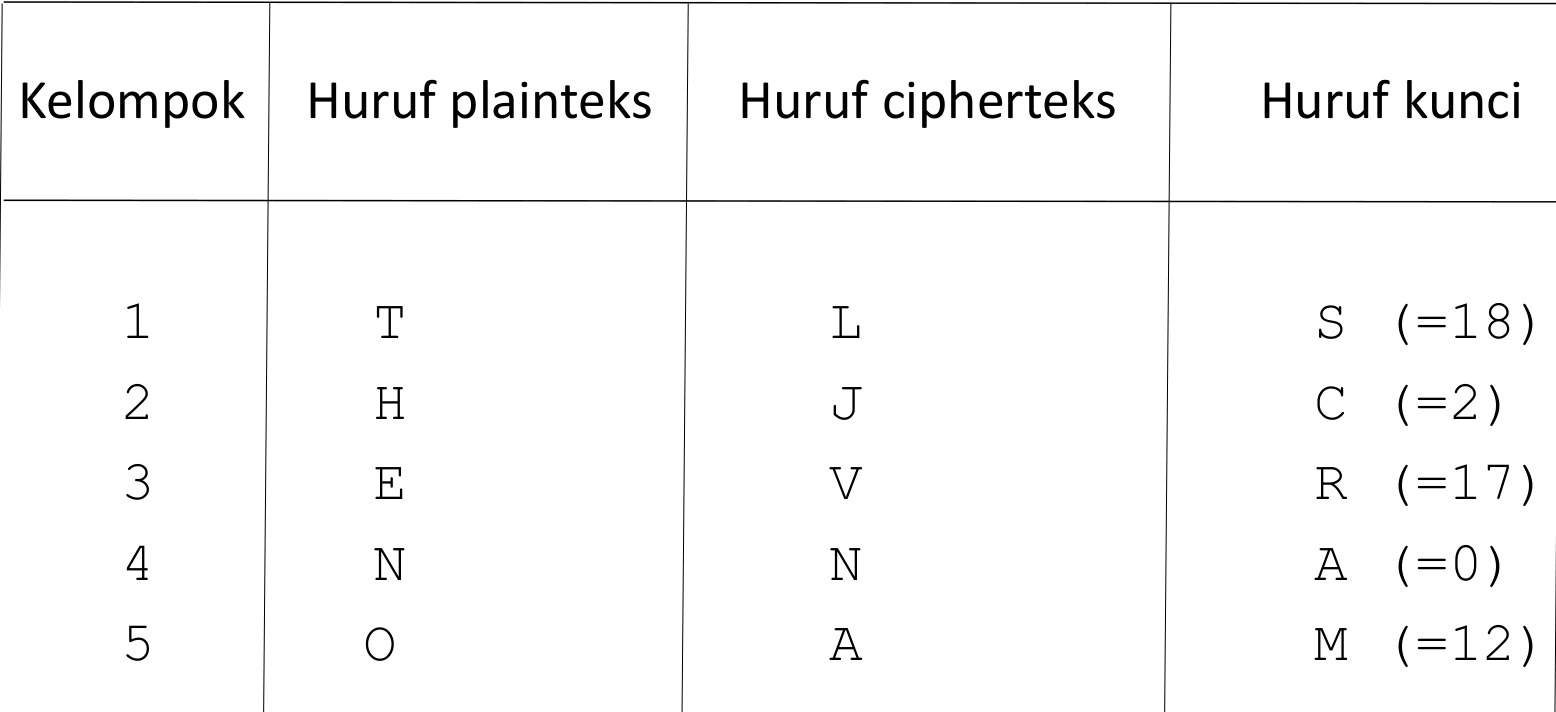
\includegraphics[width=170.10mm,height=196.02mm]{../../images/llm/page_060_img_01.png}%
\end{textblock*}

\end{document}
